\section{Polar crystals}\label{sec:5.5}

At the center of the zone the three optical phonons of silicon share one energy, \SI{64.1}{meV}. In GaAs they do not. Two transverse optical (TO) modes lie at \SI{33.6}{meV} and the longitudinal one (LO) at \SI{36.4}{meV}~\cite{strauch1990phonon}, although the three move the nuclei in the same way, gallium against arsenic, and differ only in the direction of that motion relative to $\vect{Q}$. The three energies differ because gallium and arsenic are not equivalent. When the two sublattices move against each other, every cell acquires an electric dipole. In a longitudinal wave the dipoles add up to a macroscopic polarization, whose field pulls the ions back and stiffens the mode; in a transverse wave they produce no macroscopic field. For dark matter this dipole makes a polar crystal a useful target. A dark photon couples to the dipoles coherently, cell by cell, and so does a dark-matter particle that couples to charge through a light dark photon. The charge that sets the size of the dipole is the Born effective charge.

\subsection{Born effective charges}

The fields that matter here vary over many cells. The microscopic field $\vect{E}$ of \cref{sec:1.4} oscillates within each cell, and a long wave sees its average over a cell, the \emph{macroscopic electric field} $\vect{\mathcal{E}}$, which is the $\vect{G} = 0$ component of the field in the language of \cref{sec:4.4}. The density of dipole moment, averaged over a cell in the same way, is the \emph{polarization} $\vect{P}$, and in the Heaviside--Lorentz units of the book the displacement field is $\vect{D} = \vect{\mathcal{E}} + \vect{P}$ (\cref{app:A.2}), so that the electronic dielectric constant of \cref{sec:4.4} is $\varepsilon_\infty = 1 + \partial P/\partial\mathcal{E}$ at clamped nuclei.

Now let each sublattice $\kappa$ of the crystal move rigidly by $\vect{u}_\kappa$, the zone-center displacement of \cref{eq:5.1-Fk}, in a uniform field $\vect{\mathcal{E}}$. The electrons follow the displacements and the field adiabatically. The energy per cell at fixed field, $E^{\mathrm{ad}}_{\mathcal{E}}$, reduces to the energy surface $E^{\mathrm{ad}}_{\mathrm{cell}}$ of \cref{sec:5.1} at $\vect{\mathcal{E}} = 0$. To second order in the displacements and the field, $E^{\mathrm{ad}}_{\mathcal{E}}$ is
\begin{equation}
  E^{\mathrm{ad}}_{\mathcal{E}}(u,\vect{\mathcal{E}}) = \frac12\sum_{\kappa\kappa'}\vect{u}_\kappa\cdot C^{\mathrm{an}}_{\kappa\kappa'}\cdot\vect{u}_{\kappa'} - e\sum_\kappa\vect{u}_\kappa\cdot Z^*_\kappa\cdot\vect{\mathcal{E}} - \frac\Omega2\,\vect{\mathcal{E}}\cdot(\varepsilon_\infty - 1)\cdot\vect{\mathcal{E}} ,
  \label{eq:5.5-U}
\end{equation}
with $\Omega$ the cell volume. Each coefficient is defined as a second derivative of $E^{\mathrm{ad}}_{\mathcal{E}}$. $C^{\mathrm{an}}_{\kappa\kappa'} = \sum_{\vect{R}}\Phi^{(2)}_{\kappa\kappa'}(\vect{0},\vect{R})$ is the zone-center block of the force constants of \cref{sec:5.2}, taken at zero macroscopic field; $\varepsilon_\infty$ is the electronic dielectric tensor; and the mixed derivative defines the \emph{Born effective charge} tensor $Z^*_\kappa$ of each sublattice. The first derivatives are the force on a nucleus and the polarization, $\vect{F}_\kappa = -\partial E^{\mathrm{ad}}_{\mathcal{E}}/\partial\vect{u}_\kappa$ and $\vect{P} = -\Omega^{-1}\partial E^{\mathrm{ad}}_{\mathcal{E}}/\partial\vect{\mathcal{E}}$:
\begin{equation}
  \vect{F}_\kappa = -\sum_{\kappa'}C^{\mathrm{an}}_{\kappa\kappa'}\cdot\vect{u}_{\kappa'} + e\,Z^*_\kappa\cdot\vect{\mathcal{E}} , \qquad
  \vect{P} = \frac{e}{\Omega}\sum_\kappa\vect{u}_\kappa\cdot Z^*_\kappa + (\varepsilon_\infty - 1)\cdot\vect{\mathcal{E}} .
  \label{eq:5.5-FP}
\end{equation}
The force identifies the Born charge as the force on nucleus $\kappa$ per unit uniform field. The polarization identifies the same tensor as the dipole per cell created by a unit displacement:
\begin{equation}
  e\,Z^{*,\alpha\beta}_\kappa = \frac{\partial F^\alpha_\kappa}{\partial\mathcal{E}^\beta}\bigg|_{\vect{u} = 0} = \Omega\,\frac{\partial P^\beta}{\partial u^\alpha_\kappa}\bigg|_{\vect{\mathcal{E}} = 0} .
  \label{eq:5.5-Z}
\end{equation}
The two derivatives are equal because both are the same mixed second derivative of $E^{\mathrm{ad}}_{\mathcal{E}}$; the equality is a Maxwell relation. The first Cartesian index of $Z^*_\kappa$ belongs to the force, or to the displacement, and the second to the field, or to the polarization. Some codes and papers store the transpose~\cite[Eqs.~(89)--(91)]{baroni2001phonons}; the choice of convention matters only at sites of low symmetry, since at a cubic site $Z^*_\kappa$ is a multiple of the identity.

The Born charge measures the charge that moves with a nucleus. A field acts on the bare nucleus with the force $Z_\kappa e\vect{\mathcal{E}}$, and on its electrons, which are pulled the other way and drag on the nucleus through the forces of \cref{eq:5.1-HF}. If the electrons of each atom followed their nucleus rigidly, $Z^*_\kappa$ would be the net charge of the atom. They do not: as the sublattices move, the bonds change length and electronic charge flows along them, and this flow adds to the dipole. A Born charge is therefore a dynamical quantity. It need not be an integer, and it differs from any charge one might assign to an atom by dividing up the static density, a division that has no unique answer.

The Born charges of a neutral crystal add up to zero. Displacing all sublattices together by the same $\vect{u}$, with the electrons following, translates the charge distribution of every cell. The dipole moment of a neutral distribution does not depend on where it sits, and $\vect{P}$ does not change. By \cref{eq:5.5-FP}, an unchanged $\vect{P}$ requires $\vect{u}\cdot\sum_\kappa Z^*_\kappa = 0$ for every $\vect{u}$, that is
\begin{equation}
  \sum_\kappa Z^*_\kappa = 0 ,
  \label{eq:5.5-neutral}
\end{equation}
the charge neutrality of the Born charges, also called their acoustic sum rule. In GaAs each site has tetrahedral symmetry, the two Born-charge tensors are multiples of the identity, and neutrality leaves one number, $Z^*_{\mathrm{Ga}} = -Z^*_{\mathrm{As}} \equiv Z^*$. In silicon, inversion through the bond center exchanges the two atoms and forces $Z^*_1 = Z^*_2$; neutrality then forces both charges to vanish.

The polarization in \cref{eq:5.5-Z} needs a definition. For a molecule the dipole moment is $\int\dd^3r\,\vect{r}\,\rho(\vect{r})$ with $\rho$ the charge density. For a crystal the same integral over one cell depends on where the cell boundaries are drawn, and with the periodic boundary conditions of \cref{sec:3.1} the position operator is not even well defined. Only a change of polarization is measurable: the charge per unit area that flows through the crystal while the nuclei are displaced slowly. King-Smith and Vanderbilt showed that this change is a Berry phase of the occupied Bloch states, accumulated as $\vect{k}$ crosses the zone~\cite{kingsmith1993theory}. Equivalently, the electronic polarization is $-eg_{\mathrm{deg}}/\Omega$ times the sum of the centers of the occupied Wannier functions of one cell (\cref{sec:3.6}), with $g_{\mathrm{deg}} = 2$ for spin. This \emph{Berry-phase theory} of polarization defines $\vect{P}$ only up to a quantum, a lattice vector times $e g_{\mathrm{deg}}/\Omega$, because a Wannier center can be assigned to any cell; the Born charge, a derivative, is free of that ambiguity.

The density-functional perturbation theory that yields the phonons also yields $\varepsilon_\infty$ and $Z^*_\kappa$. A uniform field enters the Sternheimer equation as one more perturbation, through the matrix elements of $\vect{r}$ between occupied and empty states, and the self-consistent solution gives the induced polarization. Either side of \cref{eq:5.5-Z} can then be evaluated, and \cref{app:E.4} describes the practice. The sum rule \cref{eq:5.5-neutral} is a cheap convergence test. In the PBE calculation behind \cref{fig:5-gaas}, the two charges of GaAs miss neutrality by \SI{12}{\percent} on the $8^3$ grid of crystal momenta used for the phonons. Only near a $28^3$ grid does their sum vanish, with $Z^* = 2.094$, within \SI{1}{\percent} of the value 2.11 that the measured LO--TO splitting implies (\cref{we:5-lst}).

The dielectric constant converges more slowly, from 26.0 on the $8^3$ grid to 13.7 on the $28^3$ grid, where successive grids differ by less than one percent. In this calculation PBE puts the direct gap of GaAs at $\mathrm{\Gamma}$ at \SI{0.57}{eV}, against the measured \SI{1.52}{eV} (\cref{tab:E-functionals}). The response to a field, built from the energy denominators of the interband transitions, is then dominated by the small region around $\mathrm{\Gamma}$ where the gap is smallest, and a coarse grid samples it poorly. The converged value is still \SI{26}{\percent} above the measured $\varepsilon_\infty = 10.88$~\cite{lockwood2005optical}. That error belongs to the functional: a gap that is too small makes the electrons too polarizable, and no numerical parameter removes the error.

\subsection{LO--TO splitting}

In \cref{eq:5.5-FP} the field is still an external parameter. In a lattice wave no one applies the field: the displaced ions create it, and it acts back on them. Let the displacements vary as $\ee^{\ii\vect{Q}\cdot\vect{r}}$, with $|\vect{Q}|$ small compared with the reciprocal-lattice vectors, so that within many cells the displacement is the uniform $\vect{u}_\kappa$ of \cref{eq:5.5-U}. We also take $|\vect{Q}|$ large compared with $\omega/c$; this condition lets us neglect retardation and use electrostatics, and we will come back to it. Two equations then fix the field. A static field has no curl, so the field of a wave is longitudinal, $\vect{\mathcal{E}} = \hat{\vect{Q}}\,\mathcal{E}_\parallel$, and there is no free charge, so $\hat{\vect{Q}}\cdot\vect{D} = 0$. With \cref{eq:5.5-FP} the second condition reads
\begin{equation*}
  \hat{\vect{Q}}\cdot\varepsilon_\infty\cdot\hat{\vect{Q}}\;\mathcal{E}_\parallel + \frac{e}{\Omega}\sum_{\kappa'}\vect{u}_{\kappa'}\cdot Z^*_{\kappa'}\cdot\hat{\vect{Q}} = 0 .
\end{equation*}
Solving for $\mathcal{E}_\parallel$ and inserting it in the force adds a matrix $C^{\mathrm{na}}_{\kappa\kappa'}(\hat{\vect{Q}})$ to the force constants:
\begin{keyresult}[Nonanalytic term of the dynamical matrix]
\begin{equation}
  D^{\mathrm{dyn},\alpha\beta}_{\kappa\kappa'}(\vect{Q}\to0) = \frac{1}{\sqrt{M_\kappa M_{\kappa'}}}\Bigl[C^{\mathrm{an},\alpha\beta}_{\kappa\kappa'} + \frac{e^2}{\Omega}\,\frac{(Z^*_\kappa\cdot\hat{\vect{Q}})^\alpha\,(Z^*_{\kappa'}\cdot\hat{\vect{Q}})^\beta}{\hat{\vect{Q}}\cdot\varepsilon_\infty\cdot\hat{\vect{Q}}}\Bigr] ,
  \label{eq:5.5-na}
\end{equation}
with $(Z^*_\kappa\cdot\hat{\vect{Q}})^\alpha = \sum_\beta Z^{*,\alpha\beta}_\kappa\hat Q^\beta$, the analytic part $C^{\mathrm{an}}$ computed at zero macroscopic field, and the masses as in \cref{eq:5.2-Ddyn}.
\end{keyresult}
This is the Heaviside--Lorentz form of the result of Gonze and Lee~\cite{gonze1997dynamical} and of Ref.~\cite[Eq.~(98)]{baroni2001phonons}, after the substitution $4\pi e^2_{\mathrm{G}} \to e^2$ of \cref{eq:A.2-map}. The second term, $C^{\mathrm{na}}$ with the masses divided out, is the \emph{nonanalytic term}. The reason for the name is that the term depends on the direction $\hat{\vect{Q}}$ from which the zone center is approached but not on $|\vect{Q}|$. The macroscopic field is the $\vect{G} = 0$ Coulomb interaction $e^2/Q^2$ acting between two dipole densities, each proportional to $\vect{Q}$, and the ratio of their product to $Q^2$ stays finite as $Q \to 0$ without having a limit. No Taylor series in $\vect{Q}$ can represent a function that depends only on the direction of $\vect{Q}$, and the dynamical matrix of a polar crystal at $\vect{Q} = 0$ is a family of matrices labeled by $\hat{\vect{Q}}$.

In a cubic crystal with two atoms per cell the consequences are explicit. There $Z^*_1 = -Z^*_2 = Z^*$ times the identity, $\varepsilon_\infty$ is a scalar, and the acoustic sum rule of \cref{sec:5.2} leaves one zone-center constant, $C^{\mathrm{an}}_{11} = C^{\mathrm{an}}_{22} = -C^{\mathrm{an}}_{12} = C_0$ times the identity. The equations of motion of the two sublattices, $M_1\ddot{\vect{u}}_1 = \vect{F}_1$ and $M_2\ddot{\vect{u}}_2 = \vect{F}_2$, then involve only the relative displacement $\vect{u}_{\mathrm{rel}} = \vect{u}_1 - \vect{u}_2$. Dividing each equation by its mass and subtracting, with $\vect{F}_1 = -C_0\vect{u}_{\mathrm{rel}} + eZ^*\vect{\mathcal{E}} = -\vect{F}_2$ from \cref{eq:5.5-FP}, gives
\begin{equation*}
  \mu_{\mathrm{red}}\,\ddot{\vect{u}}_{\mathrm{rel}} = -C_0\,\vect{u}_{\mathrm{rel}} + eZ^*\vect{\mathcal{E}}, \qquad \vect{P} = \frac{eZ^*}{\Omega}\,\vect{u}_{\mathrm{rel}} + (\varepsilon_\infty - 1)\vect{\mathcal{E}} ,
\end{equation*}
with $\mu_{\mathrm{red}} = M_1M_2/(M_1 + M_2)$ the reduced mass of the pair, as in the diatomic chain of \cref{we:5-chain}. In a transverse optical mode, $\vect{u}_{\mathrm{rel}} \perp \hat{\vect{Q}}$, the dipoles create no longitudinal field, and the frequency comes from the springs alone, $\omega_{\mathrm{T}}^2 = C_0/\mu_{\mathrm{red}}$. In the longitudinal mode, $\vect{u}_{\mathrm{rel}} \parallel \hat{\vect{Q}}$, the condition $\hat{\vect{Q}}\cdot\vect{D} = 0$ makes the field $\vect{\mathcal{E}} = -eZ^*\vect{u}_{\mathrm{rel}}/(\Omega\varepsilon_\infty)$, which opposes the displacement. The longitudinal frequency $\omega_{\mathrm{L}}$ is then higher,
\begin{equation}
  \omega_{\mathrm{L}}^2 = \omega_{\mathrm{T}}^2 + \frac{e^2Z^{*2}}{\Omega\,\varepsilon_\infty\,\mu_{\mathrm{red}}} ,
  \label{eq:5.5-LOTO}
\end{equation}
and the difference $\omega_{\mathrm{L}} - \omega_{\mathrm{T}}$ is the \emph{LO--TO splitting}. The longitudinal mode carries the electrostatic energy of its own polarization, screened by the electrons, and the Born charge enters squared, divided by $\varepsilon_\infty$. A quick estimate shows the size of the splitting. With $Z^* = 2$, $\Omega = \SI{45}{\angstrom^3}$, $\varepsilon_\infty = 11$ and $\mu_{\mathrm{red}} = \SI{36}{u}$, the second term of \cref{eq:5.5-LOTO} is $\sim\SI{2e-4}{eV^2}$, small against $\omega_{\mathrm{T}}^2 \approx \SI{1.1e-3}{eV^2}$; the splitting is a few meV, less than a tenth of the optical energy.

\begin{figure}[tbp]
  \centering
  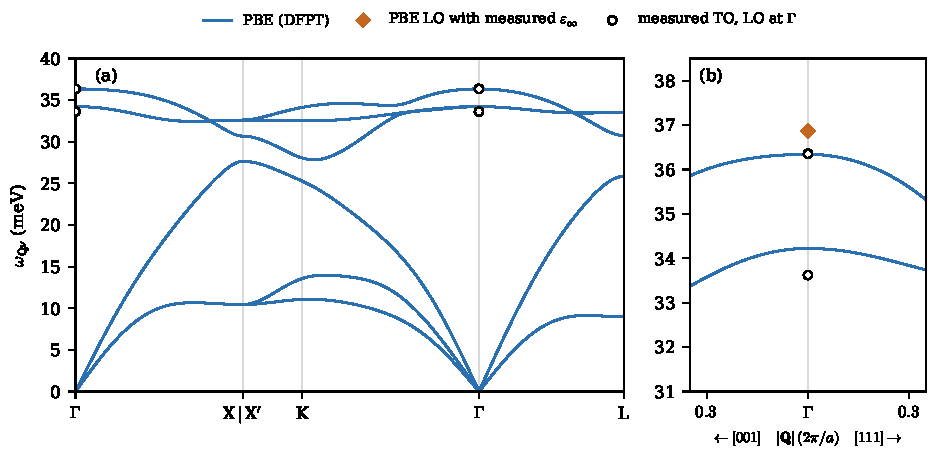
\includegraphics[width=\linewidth]{figures/ch05/fig5_4.pdf}
  \caption{Phonon dispersion of GaAs. (a) Computed along $\mathrm{\Gamma}$--X--K--$\mathrm{\Gamma}$--L with density-functional perturbation theory: PBE functional, SG15 norm-conserving pseudopotentials with the gallium $3d$ shell in the valence, a \SI{60}{Ry} cutoff, an $8^3$ grid of crystal momenta, the static-lattice constant $a = \SI{5.638}{\angstrom}$ of \cref{tab:E-functionals} (the measured value extrapolated to zero temperature with the zero-point expansion removed) and natural masses, on a $4^3$ grid of wavevectors. The force constants are Fourier interpolated with the dipole term of \cref{eq:5.5-na} subtracted and added back, using $\varepsilon_\infty = 13.7$ and $Z^* = 2.094$ computed on a $28^3$ grid of crystal momenta; acoustic sum rules imposed on the force constants and on the Born charges. Circles: measured TO and LO energies at $\mathrm{\Gamma}$, 8.13 and \SI{8.79}{THz}~\cite{strauch1990phonon}, as tabulated in Ref.~\cite[Table~I]{dehghani2025influence}. (b) Optical branches near $\mathrm{\Gamma}$ along $[001]$ (left) and $[111]$ (right), with $|\vect{Q}|$ in units of $2\pi/a$. Diamond: LO energy at $\mathrm{\Gamma}$ from \cref{eq:5.5-LOTO} with the computed TO energy and Born charge and the measured $\varepsilon_\infty = 10.88$~\cite{lockwood2005optical}.}
  \label{fig:5-gaas}
\end{figure}

\Cref{fig:5-gaas} shows the computed phonons of GaAs. The transverse optical energy at $\mathrm{\Gamma}$ comes out at \SI{34.22}{meV}, \SI{1.8}{\percent} above the measured \SI{33.62}{meV}. PBE usually makes phonons slightly soft, but here the measured lattice constant compresses the crystal relative to the PBE minimum at \SI{5.746}{\angstrom} (\cref{tab:E-functionals}). The longitudinal branch meets the zone center at \SI{36.34}{meV} from every direction. In a cubic crystal $Z^*_\kappa\cdot\hat{\vect{Q}} = Z^*_\kappa\hat{\vect{Q}}$ and $\hat{\vect{Q}}\cdot\varepsilon_\infty\cdot\hat{\vect{Q}} = \varepsilon_\infty$ for every $\hat{\vect{Q}}$, and the nonanalytic term does not depend on the direction; in an anisotropic crystal such as sapphire it does, and so does the LO frequency at $\mathrm{\Gamma}$~\cite{griffin2018directional}. The computed splitting is \SI{2.12}{meV} against the measured \SI{2.73}{meV}, \SI{22}{\percent} short, and \cref{eq:5.5-LOTO} shows why. The second term of \cref{eq:5.5-LOTO} is $e^2Z^{*2}/(\Omega\varepsilon_\infty\mu_{\mathrm{red}})$, the Born charge is right to a percent, and $\varepsilon_\infty$ is \SI{26}{\percent} too large. With the measured $\varepsilon_\infty$ and the computed $Z^*$ and $\omega_{\mathrm{T}}$, the same formula yields a splitting of \SI{2.65}{meV}, within \SI{3}{\percent} of the measurement (the diamond in \cref{fig:5-gaas}(b)). The computed LO energy itself agrees with the measured one, but by accident: the transverse energy is high and the splitting short by nearly the same amount. The near-equal masses of gallium and arsenic leave almost no gap between the acoustic and optical bands: the longitudinal acoustic branch ends at \SI{27.65}{meV} at X, and the optical band begins \SI{0.2}{meV} higher.

Because of the nonanalytic term, Fourier interpolation of the force constants needs an extra step in a polar crystal. In real space the dipole--dipole interaction behind \cref{eq:5.5-na} falls off as the inverse cube of the distance, too slowly for any grid of wavevectors to capture, and the computed $D^{\mathrm{dyn}}(\vect{Q})$ near $\mathrm{\Gamma}$ is not smooth. The analytic part $C^{\mathrm{an}}$ is the response with the $\vect{G} = 0$ term of the Coulomb interaction removed~\cite{pick1970microscopic}, and for this reason it can be computed at zero macroscopic field. Since the nonanalytic term is fixed by $Z^*_\kappa$ and $\varepsilon_\infty$ alone, it can be subtracted from the computed matrices in an Ewald-summed form that is periodic in $\vect{Q}$. The short-ranged difference between the computed matrices and this term is then interpolated, and the nonanalytic term is added back analytically at each target $\vect{Q}$~\cite{gonze1997dynamical}. \Cref{fig:5-gaas} was interpolated in this way from a $4^3$ grid.

The electrostatic treatment assumed $|\vect{Q}| \gg \omega/c$. For wavevectors comparable with $\omega/c$, the transverse optical phonon mixes with the photon of the same wavevector and frequency, and the two form the coupled modes called \emph{phonon polaritons}. The crossover happens near $Q \sim \varepsilon_0^{1/2}\omega_{\mathrm{T}}$ in natural units, about \SI{0.1}{eV} for $\omega_{\mathrm{T}} \sim \SI{30}{meV}$ and less than $10^{-4}$ of the size of the zone; at this wavevector the photon line $\omega = Q/\varepsilon_0^{1/2}$ meets the phonon. Dark-matter scattering transfers $q \sim m_\chi v \gtrsim \SI{1}{eV}$ for any mass above a keV, and for the phonons it excites the electrostatic result is exact. Absorption is different. A boson of mass $m$ from the halo, moving at $v \sim 10^{-3}$, deposits $\omega \approx m$ with a momentum of only $mv \sim 10^{-3}\omega$, deep inside the polariton region. The crystal then sees a field that is uniform in space, and the coupling to a uniform field is derived below.

\subsection{The Lyddane--Sachs--Teller relation}

A uniform field oscillating at frequency $\omega$, $\vect{\mathcal{E}}\,\ee^{-\ii\omega t}$, is the opposite limit, $Q \to 0$ at fixed $\omega$, and it measures the dielectric function of the crystal with the lattice included. The field now drives the relative displacement without any longitudinal constraint, to the steady response $\vect{u}_{\mathrm{rel}} = eZ^*\vect{\mathcal{E}}/[\mu_{\mathrm{red}}(\omega_{\mathrm{T}}^2 - \omega^2)]$, and the electrons respond with $\varepsilon_\infty$ as long as $\omega$ lies far below the gap, the adiabatic condition of \cref{sec:5.1}. Inserting $\vect{u}_{\mathrm{rel}}$ into $\vect{P}$ gives the dielectric function $\varepsilon(\omega) = D/\mathcal{E} = 1 + P/\mathcal{E}$ as
\begin{equation}
  \varepsilon(\omega) = \varepsilon_\infty + \frac{e^2Z^{*2}}{\Omega\,\mu_{\mathrm{red}}\,(\omega_{\mathrm{T}}^2 - \omega^2)}
  = \varepsilon_\infty\,\frac{\omega_{\mathrm{L}}^2 - \omega^2}{\omega_{\mathrm{T}}^2 - \omega^2} ,
  \label{eq:5.5-eps}
\end{equation}
where the second form uses \cref{eq:5.5-LOTO} to replace $e^2Z^{*2}/(\Omega\mu_{\mathrm{red}})$ by $\varepsilon_\infty(\omega_{\mathrm{L}}^2 - \omega_{\mathrm{T}}^2)$. At frequencies well above $\omega_{\mathrm{T}}$ the ions cannot follow, and $\varepsilon \to \varepsilon_\infty$; for this reason the electronic dielectric constant is also called the high-frequency dielectric constant (\cref{sec:4.4}). At $\omega = 0$ the ions follow fully and add their polarization. The \emph{static dielectric constant} $\varepsilon_0 = \varepsilon(0)$, lattice included, is $\varepsilon_\infty + e^2Z^{*2}/(\Omega\mu_{\mathrm{red}}\omega_{\mathrm{T}}^2)$, and the second form of \cref{eq:5.5-eps} turns this expression into a relation between measurable quantities alone:
\begin{keyresult}[Lyddane--Sachs--Teller relation]
\begin{equation}
  \frac{\varepsilon_0}{\varepsilon_\infty} = \frac{\omega_{\mathrm{L}}^2}{\omega_{\mathrm{T}}^2} .
  \label{eq:5.5-LST}
\end{equation}
For several polar modes, $\varepsilon_0/\varepsilon_\infty = \prod_\nu\omega_{\mathrm{L}\nu}^2/\omega_{\mathrm{T}\nu}^2$ (\cref{eq:D.14-LSTgen}).
\end{keyresult}
This is the relation of Lyddane, Sachs and Teller~\cite{lyddane1941polar}. The Born charge, the masses and the cell volume have dropped out: the ratio of the two dielectric constants is fixed by the ratio of two frequencies. The general form, with one factor per polar mode, is due to Cochran and Cowley~\cite{cochran1962dielectric}, and follows from the interlacing of the poles and zeros of $\varepsilon(\omega)$.

Those poles and zeros are the content of \cref{eq:5.5-eps}, and they hold beyond the model. The transverse frequency is a pole: a transverse mode creates no field, so it needs none, and it shows up where the response to a field diverges. The longitudinal frequency is a zero. A longitudinal mode has $\vect{\mathcal{E}} \parallel \hat{\vect{Q}}$ and needs $\hat{\vect{Q}}\cdot\vect{D} = \varepsilon(\omega)\,\mathcal{E}_\parallel = 0$, which allows a nonzero field only where $\varepsilon(\omega)$ vanishes. A zero of $\varepsilon(\omega)$ also fixes the plasmon of \cref{sec:4.5}, a self-sustained longitudinal oscillation of the electrons; the LO phonon is a self-sustained longitudinal oscillation of the ions. Between $\omega_{\mathrm{T}}$ and $\omega_{\mathrm{L}}$, \cref{eq:5.5-eps} is negative, no transverse wave propagates, and light in this band, the reststrahlen band, is reflected~\cite[Chap.~27]{ashcroft1976solid}. The loss function $\Imag[-1/\varepsilon(\omega)]$ of \cref{sec:4.4} peaks at $\omega_{\mathrm{L}}$, and the absorption $\varepsilon_2$ at $\omega_{\mathrm{T}}$, once the phonons are given a width.

With several polar modes the steps that led to \cref{eq:5.5-eps} give the general form. Let $\omega_{\mathrm{T}\nu}$ and $\vect{e}_{\kappa\nu}$ be the frequencies and polarization vectors of the analytic problem at $\vect{Q} = 0$, the eigenpairs of $C^{\mathrm{an}}_{\kappa\kappa'}/(M_\kappa M_{\kappa'})^{1/2}$, chosen real. With the expansion $\vect{u}_\kappa = \sum_\nu\vect{e}_{\kappa\nu}a_\nu/\sqrt{M_\kappa}$, each normal coordinate obeys $\ddot a_\nu = -\omega_{\mathrm{T}\nu}^2a_\nu + e\,\vect{z}_\nu\cdot\vect{\mathcal{E}}$, with the mode charge vector $\vect{z}_\nu = \sum_\kappa\vect{e}_{\kappa\nu}\cdot Z^*_\kappa/\sqrt{M_\kappa}$, and it contributes $(e/\Omega)\,a_\nu\vect{z}_\nu$ to the polarization. In a cubic crystal, along any direction $\hat{\vect{e}}$,
\begin{equation*}
  \varepsilon(\omega) = \varepsilon_\infty + \frac{e^2}{\Omega}\sum_\nu\frac{(\vect{z}_\nu\cdot\hat{\vect{e}})^2}{\omega_{\mathrm{T}\nu}^2 - \omega^2} .
\end{equation*}
This is a rational function of $\omega^2$ that tends to $\varepsilon_\infty$ at large $\omega$, has simple poles at the polar transverse frequencies, and, by the argument above, vanishes at the longitudinal frequencies $\omega_{\mathrm{L}\nu}$. Between two consecutive poles it rises monotonically from $-\infty$ to $+\infty$, and above the highest pole it rises from $-\infty$ toward $\varepsilon_\infty$, so there is exactly one zero above each pole and below the next. A rational function is fixed by its poles, its zeros and its limit at infinity, so $\varepsilon(\omega) = \varepsilon_\infty\prod_\nu(\omega_{\mathrm{L}\nu}^2 - \omega^2)/(\omega_{\mathrm{T}\nu}^2 - \omega^2)$, and at $\omega = 0$
\begin{equation}
  \frac{\varepsilon_0}{\varepsilon_\infty} = \prod_\nu\frac{\omega_{\mathrm{L}\nu}^2}{\omega_{\mathrm{T}\nu}^2} ,
  \label{eq:D.14-LSTgen}
\end{equation}
which generalizes \cref{eq:5.5-LST}.

\begin{workedexample}{The Lyddane--Sachs--Teller relation for GaAs}\label{we:5-lst}
We test \cref{eq:5.5-LST} on measured numbers. Neutron scattering puts the optical phonons of GaAs at $\omega_{\mathrm{T}} = \SI{8.13}{THz} = \SI{33.62}{meV}$ and $\omega_{\mathrm{L}} = \SI{8.79}{THz} = \SI{36.35}{meV}$~\cite{strauch1990phonon}, as tabulated in Ref.~\cite[Table~I]{dehghani2025influence}, and infrared spectroscopy measured $\varepsilon_0 = 12.9$ and $\varepsilon_\infty = 10.88$~\cite{lockwood2005optical}, as quoted in Ref.~\cite{knapen2018detection}.

\emph{The relation.} The two sides are
\begin{equation*}
  \frac{\varepsilon_0}{\varepsilon_\infty} = \frac{12.9}{10.88} = 1.186 , \qquad
  \frac{\omega_{\mathrm{L}}^2}{\omega_{\mathrm{T}}^2} = \Bigl(\frac{8.79}{8.13}\Bigr)^2 = 1.169 ,
\end{equation*}
equal to \SI{1.4}{\percent}. Read as a prediction, the relation puts the longitudinal phonon at $\omega_{\mathrm{L}} = \omega_{\mathrm{T}}(\varepsilon_0/\varepsilon_\infty)^{1/2}$, or \SI{36.61}{meV}, \SI{0.26}{meV} or \SI{0.7}{\percent} above the measurement. The splitting itself comes out as \SI{2.99}{meV} against \SI{2.73}{meV}, \SI{9}{\percent} high. The relative error grows because the ratio is close to one: $\omega_{\mathrm{L}}^2 - \omega_{\mathrm{T}}^2$ is $0.17\,\omega_{\mathrm{T}}^2$, and a \SI{1.4}{\percent} error in the ratio is a \SI{10}{\percent} error in that difference. For a harmonic crystal with adiabatic electrons the relation is exact. The \SI{1.4}{\percent} mismatch between the two sides therefore comes from the inputs. The four numbers come from different measurements on different samples, and the dielectric constants of GaAs change at the percent level between room temperature and liquid-helium temperature~\cite{griffin2018directional}.

\emph{The Born charge.} Solved for the Born charge, \cref{eq:5.5-LOTO} reads $Z^{*2} = \Omega\varepsilon_\infty\mu_{\mathrm{red}}(\omega_{\mathrm{L}}^2 - \omega_{\mathrm{T}}^2)/e^2$. With $a = \SI{5.638}{\angstrom}$, $\Omega = a^3/4 = \SI{44.80}{\angstrom^3} = \SI{5.831e-9}{eV^{-3}}$ in natural units, the masses 69.723 and \SI{74.922}{u}, so that $\mu_{\mathrm{red}} = \SI{36.11}{u} = \SI{33.64}{GeV}$, $e^2 = 4\pi\alpha = 0.0917$ and $\omega_{\mathrm{L}}^2 - \omega_{\mathrm{T}}^2 = \SI{1.910e-4}{eV^2}$,
\begin{equation*}
  Z^* = \Bigl[\frac{(5.831\times10^{-9})\times10.88\times(3.364\times10^{10})\times(1.910\times10^{-4})}{0.0917}\Bigr]^{1/2} = 2.11 .
\end{equation*}
The static constant offers a second route, since \cref{eq:5.5-eps} at $\omega = 0$ gives $\varepsilon_0 - \varepsilon_\infty = e^2Z^{*2}/(\Omega\mu_{\mathrm{red}}\omega_{\mathrm{T}}^2)$. The second route yields 2.21, \SI{5}{\percent} more: the same \SI{1.4}{\percent} inconsistency of the inputs magnified by the difference $\varepsilon_0 - \varepsilon_\infty = 2.02$. The splitting, measured directly by one experiment, is the better input.

\emph{Against the calculation.} The converged PBE Born charge, 2.094, lies \SI{0.7}{\percent} below the value just extracted, while the PBE $\varepsilon_\infty$, 13.7, lies \SI{26}{\percent} above the measurement; the error in $\varepsilon_\infty$ is why the computed splitting of \cref{fig:5-gaas} falls short. Wherever a rate needs the combination $Z^{*2}/\varepsilon_\infty$, the measured splitting, or the computed Born charge with the measured $\varepsilon_\infty$, is the input to use.
\end{workedexample}

\subsection{Coupling to a uniform field}

The middle term of \cref{eq:5.5-U}, $-e\sum_\kappa\vect{u}_\kappa\cdot Z^*_\kappa\cdot\vect{\mathcal{E}}$, is the energy of the dipoles of the displaced sublattices in the field. For a field uniform over the crystal and slow compared with the electrons, it adds a term to the nuclear Hamiltonian of \cref{eq:5.3-H}:
\begin{equation*}
  H_{\mathcal{E}}(t) = -e\sum_{\vect{R}\kappa}\vect{u}_{\vect{R}\kappa}\cdot Z^*_\kappa\cdot\vect{\mathcal{E}}(t) .
\end{equation*}
When the phonon expansion \cref{eq:5.3-u} is inserted, the lattice sum $\sum_{\vect{R}}\ee^{\ii\vect{Q}\cdot\vect{R}} = N\delta_{\vect{Q},0}$ keeps only the modes at the zone center:
\begin{equation}
  H_{\mathcal{E}}(t) = -e\sqrt{N}\sum_\nu\frac{\vect{z}_\nu\cdot\vect{\mathcal{E}}(t)}{\sqrt{2\omega_{0\nu}}}\,B_{0\nu} ,
  \qquad
  \vect{z}_\nu = \sum_\kappa\frac{\vect{e}_{\kappa\nu}(0)\cdot Z^*_\kappa}{\sqrt{M_\kappa}} ,
  \label{eq:5.5-HE}
\end{equation}
with $\vect{z}_\nu$ the mode charge vector and $\omega_{0\nu}$ the frequency of branch $\nu$ at $\mathrm{\Gamma}$. The amplitude to create one phonon from the ground state, by \cref{eq:5.3-me}, is $-e\sqrt N\,\vect{z}_\nu\cdot\vect{\mathcal{E}}/\sqrt{2\omega_{0\nu}}$.

In \cref{eq:5.5-HE} the acoustic modes do not couple. At $\mathrm{\Gamma}$ their polarization vectors are $(M_\kappa/M_{\mathrm{cell}})^{1/2}\hat{\vect{e}}$ (\cref{sec:5.2}), so that $\vect{z}_\nu = \hat{\vect{e}}\cdot\sum_\kappa Z^*_\kappa/\sqrt{M_{\mathrm{cell}}}$, which vanishes by the charge neutrality \cref{eq:5.5-neutral}: a uniform field cannot push a neutral crystal. In GaAs the optical modes at $\mathrm{\Gamma}$ have $\vect{e}_{1} = (M_2/M_{\mathrm{cell}})^{1/2}\hat{\vect{e}}$ and $\vect{e}_{2} = -(M_1/M_{\mathrm{cell}})^{1/2}\hat{\vect{e}}$, and the same algebra as in \cref{app:D.14} leads to $\vect{z}_\nu = Z^*\hat{\vect{e}}/\sqrt{\mu_{\mathrm{red}}}$: the field couples to the optical mode polarized along it, through the Born charge and the reduced mass. The squared amplitude is proportional to $N$. All cells are driven in phase, the whole crystal absorbs the quantum, and the rate grows with the target mass, as for the single-phonon amplitude of \cref{sec:5.3}, without the momentum transfer that a scattering process has to supply.

Which resonance a probe excites depends on what it holds fixed. A field $\vect{\mathcal{E}}$ imposed inside the crystal drives the transverse resonance, the pole of $\varepsilon$ at $\omega_{\mathrm{T}}$. A probe that fixes the source of $\vect{D}$, as a moving charge does, sees $1/\varepsilon$ and excites the longitudinal mode at the zero of $\varepsilon$, $\omega_{\mathrm{L}}$. A dark photon couples through its in-medium mixing with the photon. For a dark photon at rest, of mass $m = \omega$, the medium screens that mixing by $1/\varepsilon(\omega)$: the absorption rate is the photon absorption $\omega\Imag\varepsilon$ times the screened coupling $1/|\varepsilon|^2$, and so proportional to the loss function $\Imag[-1/\varepsilon(\omega)]$~\cite[Eqs.~(2) and~(3)]{knapen2018detection}, which peaks at the zero of $\varepsilon$, $\omega_{\mathrm{L}}$. The absorption of dark-photon dark matter in GaAs therefore peaks at the LO energy, and \cref{chap:11} works out the rate. The longitudinal field also acts on the electrons. Its potential, which grows as $1/Q$ at small $Q$, is the Fr\"ohlich coupling, with a strength set by $\omega_{\mathrm{L}}$ and $1/\varepsilon_\infty - 1/\varepsilon_0$ (\cref{eq:6.2-frohlich}).

The five numbers of this section, $Z^*$, $\varepsilon_\infty$, $\varepsilon_0$, $\omega_{\mathrm{T}}$ and $\omega_{\mathrm{L}}$, obey two relations, \cref{eq:5.5-LOTO,eq:5.5-LST}, so that any three fix the other two.
